\documentclass[a4paper]{article}
\usepackage{amsmath}
\usepackage{multicol}
\usepackage{graphicx}

\title{Advanced Concepts of Machine Learning: Sparse Autoencoder}
\author{Kevin Trebing (i6192338), Alberto Perez (i6201157)}

\begin{document}
\maketitle

\section{How to use}

Execute the python file \textit{sparse\_autoencoder.py} with python3. An optimization will run that trains the autoencoder. Different parameters can be chosen, such as the learning rate $\alpha$ (called ALPHA) with default value $1.5$ and $\lambda$ (called LAMBDA) with default value $0.00005$. Furthermore, the training stops when the total error of one epoch (i.e. seeing each training sample once) is below a certain threshold (default for this is $0.0005$).

\section{Learning performance}
The network needs about $15.000-20.000$ epochs to converge. Note that it still does not learn the mapping perfectly, instead of zeros it most often leads to values around zero. The same goes for values of one, here it leads to values around one. The time until convergence is about 10 seconds.

\section{Parameters}

For higher values of alpha, it is more likely that the system will converge at the wrong stability point. For high values, decreasing the size of the error used for determining convergence can decrease the chances of wrong stability points. However this also requires many iterations to achieve convergence.

The highest alpha value which admits for a reasonable amount of convergence is 5. For such a value, convergence does not take more than 2000 epochs, however sometimes the loop can go on for indefinite time. Reducing the value of alpha to around 0.8 gives a  more robust probability of  convergence. However obtaining this convergence usually takes longer. Adding a regularisation term reduces the time taken to converge; this is represented by lambda. However the main goal of the regularisation term is to avoid overfitting by trying to keep the weights to smaller magnitudes.

Lambda is not very useful for large values of alpha (where convergence is quick already). However for small values of alpha ($<$0.8), lambda can lead to a faster convergence (for example reducing the epochs necessary by one order of magnitude). This does incur a penalty as the network loses some preciseness. However, as long as the lambda is not too large ($<$0.001), the output values of the network can correctly identify the input values.

\begin{figure}
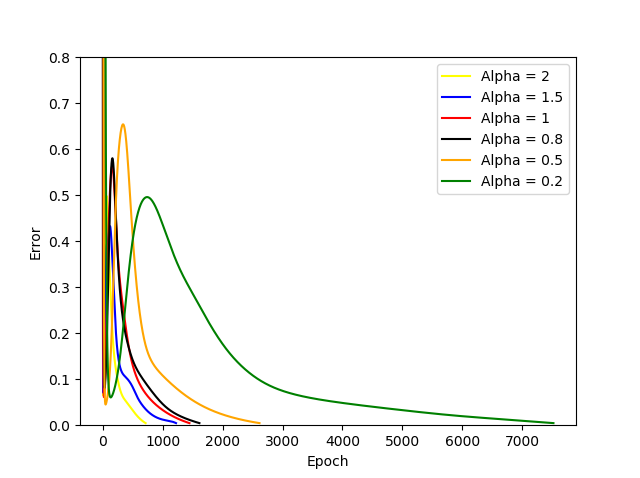
\includegraphics[scale=0.7]{learning_rate}
\caption{Different alpha values lead to different convergence speeds. The regularisation factor was fixed at 0.001.}
\end{figure}

%Adding up errors might mean positive and negative errors are cancelling each other out?

\section{Interpretation of the learned weights}

The weight matrix going from the input layer to the hidden layer has 27 weights (9 x 3) and the weight matrix going from the hidden layer to the output layer has 32 weights (4 x 8). This makes a total of 59 weights. From inspection approximately half of the value in the weights will be negative (but not necessarily exactly half of them are negative).

In a forward pass from one layer to the next, the magnitude of each weight indicates how much importance to give to each value from the input layer (of that pass). The sign indicates wether the input is adding positively or subtracting from the output value. Each weight is used once in one forward pass from one layer to the next, as there is one weight for each possible combination of inputs and outputs. In the backward propagation the magnitude of the weights indicate how much importance to give to the error found at the output activation values (relative to each original input node). 

In the forward pass all the input activations (and the bias) are multiplied by the weights going to a specific output activation (and incoming from each different input), i.e. for activation a3, it would be weights $W_{3i}$... $W_{3n}$. However in the backward pass the errors are multiplied by the weights indicating they originate from a specific node (while the errors are incoming from each different output node), i.e. for the error at activation a2, it would be weights $W_{i2}$... $W_{n2}$. 

The weights are also used when calculating the regularisation. The effect of the regularisation is to try and diminish the current behaviour of each weight. A large positive weight will have its value decreased, while a large negative weight will have its value increased. A similar effect effect will be seen in smaller weights but at a smaller scale. The overall effect is an increment on the changes the update might inflict opposing the current pattern of behaviour of the weights. The regularisation tends to create weights with a smaller magnitude when compared to the same run with no regularisation (which makes sense as the regularisation is opposing the growth of the magnitude of the weights).

When looking at the three neurons in the hidden layer we can see that an (almost) binary representation was learned. A human interpretation could be that if a neuron has an activation bigger than 0.1 we regard it as firing. Then we have a perfect binary encoding of the input.

\end{document}
